%%%%%%%%%%%%%%%%%%%%%%%%%%%%%%%%%%%%%%%%%%%%%%%%%%%%%%%%%%%%%%%%%%%%%%%%%%%%%%%%
%% Plantilla de memoria en LaTeX para la ETSIT - Universidad Rey Juan Carlos
%%
%% Por Gregorio Robles <grex arroba gsyc.urjc.es>
%%     Grupo de Sistemas y Comunicaciones
%%     Escuela Técnica Superior de Ingenieros de Telecomunicación
%%     Universidad Rey Juan Carlos
%% (muchas ideas tomadas de Internet, colegas del GSyC, antiguos alumnos...
%%  etc. Muchas gracias a todos)
%%
%% La última versión de esta plantilla está siempre disponible en:
%%     https://github.com/gregoriorobles/plantilla-memoria
%%
%% Para obtener PDF, ejecuta en la shell:
%%   make
%% (las imágenes deben ir en PNG o JPG)

%%%%%%%%%%%%%%%%%%%%%%%%%%%%%%%%%%%%%%%%%%%%%%%%%%%%%%%%%%%%%%%%%%%%%%%%%%%%%%%%

\documentclass[a4paper, 12pt]{book}
\usepackage[T1]{fontenc}

\usepackage[a4paper, left=2.5cm, right=2.5cm, top=3cm, bottom=3cm]{geometry}
\usepackage{times}
\usepackage[utf8]{inputenc}
%\usepackage[latin-1]{inputenc}
\usepackage[spanish]{babel} % Comenta esta línea si tu memoria es en inglés
\usepackage{url}
%\usepackage[dvipdfm]{graphicx}
\usepackage{graphicx}
\usepackage{float}  %% H para posicionar figuras
\usepackage[nottoc, notlot, notlof, notindex]{tocbibind} %% Opciones de índice
\usepackage{latexsym}  %% Logo LaTeX

\title{Memoria del Proyecto Fin de Carrera "Conference Book Generator"}
\author{Seila Oliva Muñoz}

\renewcommand{\baselinestretch}{1.5}  %% Interlineado

\begin{document}

\renewcommand{\refname}{Bibliografía}  %% Renombrando
\renewcommand{\appendixname}{Apéndice}

%%%%%%%%%%%%%%%%%%%%%%%%%%%%%%%%%%%%%%%%%%%%%%%%%%%%%%%%%%%%%%%%%%%%%%%%%%%%%%%%
% PORTADA

\begin{titlepage}
\begin{center}
\begin{tabular}[c]{c c}
%
\includegraphics[bb=0 0 194 352, scale=0.25]{logo} &

\includegraphics[scale=0.25]{img/logo_vect.png} &
\begin{tabular}[b]{l}
\Huge
\textsf{UNIVERSIDAD} \\
\Huge
\textsf{REY JUAN CARLOS} \\
\end{tabular}
\\
\end{tabular}

\vspace{3cm}

\Large
GRADO DE INGENIERÍA EN TECNOLOGÍAS DE LA TELECOMUNICACIÓN

\vspace{0.4cm}

\large
Curso Académico 2017/2018

\vspace{0.8cm}

Trabajo Fin de Grado

\vspace{2.5cm}

\LARGE
CONFERENCE BOOK GENERATOR

\vspace{4cm}

\large
Autor : Seila Oliva Muñoz \\
Tutor : Dr. Gregorio Robles
\end{center}
\end{titlepage}

\newpage
\mbox{}
\thispagestyle{empty} % para que no se numere esta pagina


%%%%%%%%%%%%%%%%%%%%%%%%%%%%%%%%%%%%%%%%%%%%%%%%%%%%%%%%%%%%%%%%%%%%%%%%%%%%%%%%
%%%% Para firmar
\clearpage
\pagenumbering{gobble}
\chapter*{}

\vspace{-4cm}
\begin{center}
\LARGE
\textbf{Trabajo Fin de Grado}

\vspace{1cm}
\large
Conference Book Generator

\vspace{1cm}
\large
\textbf{Autor :} Seila Oliva Muñoz \\
\textbf{Tutor :} Dr. Gregorio Robles Martínez

\end{center}

\vspace{1cm}
La defensa del presente Proyecto Fin de Carrera se realizó el día \qquad$\;\,$ de \qquad\qquad\qquad\qquad \newline de 2018, siendo calificada por el siguiente tribunal:


\vspace{0.5cm}
\textbf{Presidente:}

\vspace{1.2cm}
\textbf{Secretario:}

\vspace{1.2cm}
\textbf{Vocal:}


\vspace{1.2cm}
y habiendo obtenido la siguiente calificación:

\vspace{1cm}
\textbf{Calificación:}


\vspace{1cm}
\begin{flushright}
Fuenlabrada, a \qquad$\;\,$ de \qquad\qquad\qquad\qquad de 2018
\end{flushright}

%%%%%%%%%%%%%%%%%%%%%%%%%%%%%%%%%%%%%%%%%%%%%%%%%%%%%%%%%%%%%%%%%%%%%%%%%%%%%%%%
%%%% Dedicatoria

\chapter*{}
\pagenumbering{Roman} % para comenzar la numeracion de paginas en numeros romanos
\begin{flushright}
\textit{Dedicado a \\
mi familia / mi abuelo / mi abuela}
\end{flushright}

%%%%%%%%%%%%%%%%%%%%%%%%%%%%%%%%%%%%%%%%%%%%%%%%%%%%%%%%%%%%%%%%%%%%%%%%%%%%%%%%
%%%% Agradecimientos

\chapter*{Agradecimientos}
%\addcontentsline{toc}{chapter}{Agradecimientos} % si queremos que aparezca en el índice
\markboth{AGRADECIMIENTOS}{AGRADECIMIENTOS} % encabezado

Aquí vienen los agradecimientos\ldots Aunque está bien acordarse de la pareja, no hay que olvidarse de dar las gracias a tu madre, que aunque a veces no lo parezca disfrutará tanto de tus logros como tú\ldots
Además, la pareja quizás no sea para siempre, pero tu madre sí.

%%%%%%%%%%%%%%%%%%%%%%%%%%%%%%%%%%%%%%%%%%%%%%%%%%%%%%%%%%%%%%%%%%%%%%%%%%%%%%%%
%%%% Resumen

\chapter*{Resumen}
%\addcontentsline{toc}{chapter}{Resumen} % si queremos que aparezca en el índice
\markboth{RESUMEN}{RESUMEN} % encabezado

Aquí viene un resumen del proyecto. Ha de constar de tres o cuatro párrafos, donde se presente de manera clara y concisa de qué va el proyecto.
Han de quedar respondidas las siguientes preguntas:

\begin{itemize}
  \item ¿De qué va este proyecto? ¿Cuál es su objetivo principal?
  \item ¿Cómo se ha realizado? ¿Qué tecnologías están involucradas?
  \item ¿En qué contexto se ha realizado el proyecto? ¿Es un proyecto
dentro de un marco general?
\end{itemize}

Lo mejor es escribir el resumen al final.

%%%%%%%%%%%%%%%%%%%%%%%%%%%%%%%%%%%%%%%%%%%%%%%%%%%%%%%%%%%%%%%%%%%%%%%%%%%%%%%%
%%%% Resumen en inglés

\chapter*{Summary}
%\addcontentsline{toc}{chapter}{Summary} % si queremos que aparezca en el índice
\markboth{SUMMARY}{SUMMARY} % encabezado

Here comes a translation of the ``Resumen'' into English. Please, double check it for correct grammar and spelling.
As it is the translation of the ``Resumen'', which is supposed to be written at the end, this as well should be filled out
just before submitting.


%%%%%%%%%%%%%%%%%%%%%%%%%%%%%%%%%%%%%%%%%%%%%%%%%%%%%%%%%%%%%%%%%%%%%%%%%%%%%%%%
%%%%%%%%%%%%%%%%%%%%%%%%%%%%%%%%%%%%%%%%%%%%%%%%%%%%%%%%%%%%%%%%%%%%%%%%%%%%%%%%
% ÍNDICES %
%%%%%%%%%%%%%%%%%%%%%%%%%%%%%%%%%%%%%%%%%%%%%%%%%%%%%%%%%%%%%%%%%%%%%%%%%%%%%%%%

% Las buenas noticias es que los índices se generan automáticamente.
% Lo único que tienes que hacer es elegir cuáles quieren que se generen,
% y comentar/descomentar esa instrucción de LaTeX.

%%%% índice de contenidos
\tableofcontents
%%%% índice de figuras
\cleardoublepage
%\addcontentsline{toc}{chapter}{Lista de figuras} % para que aparezca en el indice de contenidos
\listoffigures % indice de figuras
%%%% índice de tablas
%\cleardoublepage
%\addcontentsline{toc}{chapter}{Lista de tablas} % para que aparezca en el indice de contenidos
%\listoftables % indice de tablas


%%%%%%%%%%%%%%%%%%%%%%%%%%%%%%%%%%%%%%%%%%%%%%%%%%%%%%%%%%%%%%%%%%%%%%%%%%%%%%%%
%%%%%%%%%%%%%%%%%%%%%%%%%%%%%%%%%%%%%%%%%%%%%%%%%%%%%%%%%%%%%%%%%%%%%%%%%%%%%%%%
% INTRODUCCIÓN %
%%%%%%%%%%%%%%%%%%%%%%%%%%%%%%%%%%%%%%%%%%%%%%%%%%%%%%%%%%%%%%%%%%%%%%%%%%%%%%%%

\cleardoublepage
\chapter{Introducción}
\label{chap:intro} % etiqueta para poder referenciar luego en el texto con ~\ref{sec:intro}
\pagenumbering{arabic} % para empezar la numeración de página con números

\section{Motivación}
\label{sec:motivacion}
Hoy en día es muy frecuente la realización de seminarios o conferencias de muy diversos temas. A ellos acude gente de diferentes partes del mundo, con perfiles similares o diferentes, dispuestos a aumentar su lista de contactos. \\

Normalmente, la única manera de conocer gente en estos lugares es presentándose personalmente a cada persona, y en una conferencia con un número grande de personas esta labor puede resultar tediosa, por no decir prácticamente imposible.\\

Por esto, mi tutor, Gregorio, me contó la idea de crear un ``Book'' o revista en el que apareciesen los datos de todos los asistentes a la conferencia, para repartirlo en el lugar, y así tener el contacto de todos. En este libro cada asistente podrá incluir sus datos de contacto, su centro de trabajo, sus intereses, etc.\\

Este proyecto pretende automatizar la labor de hacer este Book, de manera que cada asistente rellene un formulario previamente con sus datos, y que el documento se genere automáticamente.


\section{Estructura de la memoria}
\label{sec:estructura}

Con el fin de facilitar la lectura de la memoria, en esta sección se detalla la estructura de la misma y el contenido que se trata en cada una de las secciones:
\begin{itemize}
  \item \textbf{Capítulo \ref{chap:intro} Introducción.} Contexto en el que surge la idea del proyecto y breve explicación de la estructura de la memoria.

  \item \textbf{Capítulo \ref{chap:objetivos}: Objetivos.} En esta sección se explican los objetivos marcados durante la realización del proyecto.

  \item \textbf{Capítulo \ref{chap:estadoarte}: Estado del arte.} Presentación de las tecnologías con las que se ha desarrollado el proyecto.

  \item \ldots
\end{itemize}



%%%%%%%%%%%%%%%%%%%%%%%%%%%%%%%%%%%%%%%%%%%%%%%%%%%%%%%%%%%%%%%%%%%%%%%%%%%%%%%%
%%%%%%%%%%%%%%%%%%%%%%%%%%%%%%%%%%%%%%%%%%%%%%%%%%%%%%%%%%%%%%%%%%%%%%%%%%%%%%%%
% OBJETIVOS %
%%%%%%%%%%%%%%%%%%%%%%%%%%%%%%%%%%%%%%%%%%%%%%%%%%%%%%%%%%%%%%%%%%%%%%%%%%%%%%%%

\cleardoublepage % empezamos en página impar
\chapter{Objetivos} % título del capítulo (se muestra)
\label{chap:objetivos} % identificador del capítulo (no se muestra, es para poder referenciarlo)

\section{Objetivo general} % título de sección (se muestra)
\label{sec:objetivo-general} % identificador de sección (no se muestra, es para poder referenciarla)

El objetivo de este proyecto es crear un recurso para que todas las personas que asistan a una conferencia/seminario puedan conocer al resto de asistentes, así como darse a conocer ellos mismos, y de esta forma poder obtener información sobre cada uno (datos de contacto, situación laboral \ldots).\\

Para ello, se persigue otro objetivo que es automatizar esta labor: crear un programa que sea capaz de tomar como entrada los datos de cada asistente y generar un documento con toda la información.


\section{Objetivos específicos}
\label{sec:objetivos-especificos}

Los objetivos específicos que llevé a cabo a lo largo del proyecto fueron los siguientes:
\begin{itemize}
  \item \textbf{Trabajar con Google Forms.} Los datos de los asistentes se obtendrán de un Google Form, del que previamente se habrá recibido un enlace. Una vez recopilada toda la información, se generará una Google Sheet con ella.
  \item \textbf{Trabajar con Google Sheet API.} Para tratar la Google Sheet mencionada anteriormente, necesitaré conocer el funcionamiento de \textit{Google Sheet API}\footnote{\url{https://developers.google.com/sheets/guides/concepts?hl=es-419}} para poder extraer los datos de la \textit{Sheet} y trabajar con ellos.
  \item \textbf{Obtener todos los datos en orden y tratarlos.} Tendré que examinar todos los datos por si hay alguno que tenga que tener un trato especial (url de imágenes que habrá que descargar, textos demasiado largos que habrá que limitar, etc).
  \item \textbf{Trabajar con \LaTeX.} Una vez obtenidos todos los datos, se generará con ellos un documento \LaTeX, a partir del cual se producirá un PDF con el resultado final.
  \item \textbf{Diseñar una estructura.} Diseñar como quedará el resultado final, para generar el \LaTeX\  con esta forma.
\end{itemize}

\section{Planificación temporal}
\label{sec:planificacion-temporal}

La realización de este proyecto me ha ocupado todo un curso acadámico (9 meses), y las fases que he seguido han sido las siguientes:
\begin{itemize}
	\item \textbf{Idea de proyecto.} En primer lugar, me reuní con mi tutor del proyecto, Gregorio, para que me ayudase a elegir un proyecto que se adaptase a lo que estaba buscando. Una vez decidido el proyecto, tomé un tiempo para estudiarlo y saber qué tecnologías iba a necesitar para su desarrollo.
	\item \textbf{Aprendizaje de las tecnologías utilizadas.} Una vez me dí cuenta de las tecnologías necesarias, comencé por aprender sobre ellas: para qué sirven, cómo utilizarlas \ldots Este proceso es imprescindible para la continuación del proyecto.
	\item \textbf{Desarrollo del proyecto.} Desarrollo del código en Python para conseguir las ideas anteriormente expuestas.
	\item \textbf{Redacción de la memoria.} Como último paso del proyecto, comencé a escribir esta memoria en la que se recopilan en detalle todos los pasos que seguí para la consecución del proyecto.
\end{itemize}


%%%%%%%%%%%%%%%%%%%%%%%%%%%%%%%%%%%%%%%%%%%%%%%%%%%%%%%%%%%%%%%%%%%%%%%%%%%%%%%%
%%%%%%%%%%%%%%%%%%%%%%%%%%%%%%%%%%%%%%%%%%%%%%%%%%%%%%%%%%%%%%%%%%%%%%%%%%%%%%%%
% ESTADO DEL ARTE %
%%%%%%%%%%%%%%%%%%%%%%%%%%%%%%%%%%%%%%%%%%%%%%%%%%%%%%%%%%%%%%%%%%%%%%%%%%%%%%%%

\cleardoublepage
\chapter{Estado del arte}
\label{chap:estadoarte} % identificador del capítulo (no se muestra, es para poder referenciarlo)

En esta sección, se describen las tecnologías utilizadas para la realización del proyecto:

\section{Python}
\label{sec:python}

Python\footnote{\url{https://www.python.org/}} es un lenguaje de programación que busca la simplicidad y facilidad, así como la legibilidad del código. Es un lenguaje interpretado, es decir, no necesita ser compilado para ejecutar.\\

Con Python se pueden hacer todo tipo de programas. Aunque no es un lenguaje específico para el desarrollo web, sí se pueden desarrollar páginas con él.\\

Es un lenguaje multiparadigma: permite más de un estilo de programación (orientada a objetos, imperativa, funcional \ldots). También es multiplataforma, por lo que se puede usar con distintos sistemas informáticos.\\

Una ventaja de Python es que cuenta con un gran número de funciones incorporadas en el lenguaje (por ejemplo, para tratar strings, ficheros\ldots) y librerías para usos específicos que podemos importar a nuestro programa.


\section{Latex}
\label{sec:latex}
\LaTeX\footnote{\url{https://www.latex-project.org/}} es un sistema de composición de textos (de software libre), orientado especialmente a la creación de libros y documentos científicos y técnicos que contengan fórmulas matemáticas. Está formado por un gran conjunto de macros de TeX, con la intención de facilitar el uso del lenguaje de composición tipogrífica, TeX.\\

Una de las ventajas de \LaTeX es la calidad profesional de los documentos que genera, así como su excelente calidad de imprenta. Otra ventaja es que permite separar claramente el contenido y el formato del documento.\\

\LaTeX presupone una filosofía de trabajo diferente a la de los procesadores de texto habituales (``lo que ves es lo que obtienes'') y se basa en instrucciones. Tradicionalmente, este aspecto se ha considerado una desventaja. Sin embargo, \LaTeX permite a quien escribe un documento centrarse exclusivamente en el contenido, sin tener que preocuparse de los detalles del formato.


\section{Google Forms}
\label{sec:googleforms}
Google Forms\footnote{\url{https://www.google.es/intl/es/forms/about/}} es una herramienta útil que permite planificar eventos, enviar una encuesta, hacer preguntas o recopilar otro tipo de información de forma fácil y sencilla.\\

Crear un formulario es tan fácil como añadir las preguntas seleccionando en cada uno el tipo que mejor se adapte a nuestras necesidades. Los tipos de pregunta que nos podemos encontrar son, por ejemplo, texto, tipo test, elegir de listas, desplegables, etc. También permite añadir imágenes, videos o saltos de página para dividir la encuesta en secciones.\\

Una vez enviado el formulario a los destinatarios, se irán recopilando las respuestas recibidas. Éstas se pueden guardar en el propio Google Forms, de manera que se mostrarán como un resumen de las respuestas, o se pueden exportar a una hoja de cálculo en la que cada línea estarán las respuestas de cada persona (cada respuesta en una columna).


\section{Google Sheets API}
\label{sec:googlesheet}

Google Sheets API\footnote{\url{https://developers.google.com/sheets/api/}} permite leer y modificar cualquier aspecto de una hoja de cálculo.\\

Para utilizar esta herramienta en Python, tendremos que descargar la libreria de Google Client (\verb"pip install --upgrade google-api-python-client"), así como las credenciales necesarias.\\

Para leer el contenido de las celdas, que es lo que interesa en este caso, se utiliza la colección \textbf{spreadsheets.values}\footnote{\url{https://forward2.herokuapp.com/developers/sheets/api/reference/rest/v4/spreadsheets.values?hl=es-419}}. Con esta colección podremos especificar el rango, o rangos, de celdas que nos interesa leer (o escribir).


%%%%%%%%%%%%%%%%%%%%%%%%%%%%%%%%%%%%%%%%%%%%%%%%%%%%%%%%%%%%%%%%%%%%%%%%%%%%%%%%
%%%%%%%%%%%%%%%%%%%%%%%%%%%%%%%%%%%%%%%%%%%%%%%%%%%%%%%%%%%%%%%%%%%%%%%%%%%%%%%%
% DISEÑO E IMPLEMENTACIÓN %
%%%%%%%%%%%%%%%%%%%%%%%%%%%%%%%%%%%%%%%%%%%%%%%%%%%%%%%%%%%%%%%%%%%%%%%%%%%%%%%%

\cleardoublepage
\chapter{Diseño e implementación}

\section{Arquitectura general}
\label{sec:arquitectura}
En la figura \ref{fig:esquema} se puede observar un esquema a modo de resúmen del proceso que sigue el proyecto. A continuación, describiré cada bloque de este esquema.

\begin{figure}[h!]
	\centering
	\includegraphics[width=12cm, keepaspectratio]{Esquema2}
	\caption{Esquema de funcionamiento}
	\label{fig:esquema}
\end{figure}


\section{Creación de un formulario (Google Forms)}
\label{sec:formulario}
La base para obtener un buen resultado final, es crear desde el inicio un buen formulario. Para ello, hay que anticiparse a las respuestas de las personas que van a rellenar nuestra encuesta y, para esto, Google Forms nos ayuda mucho, ya que nos permite elegir entre múltiples tipos de respuestas posibles.\\

Por ejemplo, si preguntamos el nombre de la persona, elegiremos como tipo de respuesta la opción \textbf{Respuesta corta}, ya que el nombre consta de pocas palabras. En cambio, si pedimos una descripción, convendría elegir la opción \textbf{Párrafo} (incluso se puede limitar el número de caracteres de dicho párrafo). En los casos en los que conocemos de antemano las posibles respuestas de los asistentes, y éstas se vayan a repetir entre varios de ellos, podemos elegir las opciones de \textbf{Casillas de verificación}, \textbf{Selección múltiple} o \textbf{Desplegable}, según creamos conveniente. Algunos ejemplos de estos casos serían unas casillas de verificación para respuestas de Sí/No, o un desplegable para elegir la nacionalidad de la persona.\\

Con estos últimos casos, conseguiremos que todas las respuestas sean concisas y uniformes. Si no lo hacemos de esta forma y preguntamos, por ejemplo, ``¿Cuál es tu mes de nacimiento?'', dos personas distintas que hayan nacido en el mismo mes pueden contestar ``Yo nací en enero'' y ``Mi mes de nacimiento es enero''. Sin embargo, si aquí elegimos como tipo de respuesta un desplegable en el que simplemente haya que seleccionar el mes, obtendremos en ambas respuestas ``Enero''. Esto nos puede ayudar en el futuro si queremos, por ejemplo, buscar a todas las personas que tengan la misma respuesta a una determinada pregunta.\\

Además de estas, hay varias opciones más para las respuestas.


\section{Traspaso de respuestas a hoja de cálculo}
\label{sec:pasaraExcel}
Una vez que los participantes han rellenado el formulario, podemos acceder a sus respuestas de varias maneras: en la propia página de las preguntas, donde se pueden ver tanto las respuestas individuales como un resumen de las respuestas globales; y exportando las respuestas a una hoja de cálculo.\\

Realizaremos esta última opción, de manera que todos los datos quedarán volcados en una hoja de cálculo de Google. Esta hoja de cálculo tendrá la siguiente estructura:
\begin{itemize}
	\item En la primera fila aparece en cada celda una pregunta de las realizadas, a excepción de la primera celda, llamada ``Timestamp'', que indicará la fecha y hora a la que ha contestado cada participante.
	\item En cada una de las siguientes filas, aparecerá bajo cada pregunta la correspondiente respuesta de un participante.
\end{itemize}


\section{Extracción de los valores de la hoja de cálculo}
\label{sec:extraerExcel}
Esta es la primera parte que pertenece a mi proyecto. Lo primero que hace es obtener las credenciales necesarias para utilizar la API de Google Sheet. Una vez acreditado, con la URL de la hoja de cálculo que hemos obtenido del formulario, procedemos a la extracción de todos los datos. En este caso, no necesitamos la primera fila, donde aparecen los enunciados de las preguntas, por lo que indicaremos en el programa que queremos la información a partir de la celda 'A2'.\\

El resultado de este proceso será un array en el que cada elemento será otro array. Es decir, cada fila de la hoja de cálculo, se convertirá en un array cuyos elementos serán cada respuesta (cada celda). Estas filas (array) se guardan a su vez en otro array, quedando este último como un array de filas. Esta descripción se puede entender mejor con el siguiente ejemplo:

\begin{figure}[h!]
	\centering
	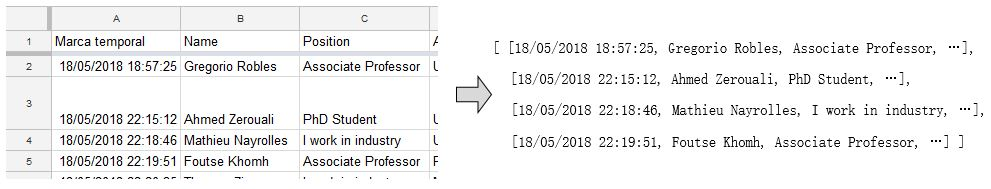
\includegraphics[width=17cm, keepaspectratio]{img/ejemplo45real}
	\caption{Ejemplo hoja de cálculo a array}
	\label{fig:ejemplo4_5}
\end{figure}

\subsection{Volcado de valores a NamedTuple}
\label{subsec:namedtuple}
Una vez tenemos el array con todos los datos, convertiremos este \textit{array de arrays} en un \textit{array de NamedTuples}.\\

NamedTuple es una \textit{``Tupla con nombre''}. Tiene una estructura parecida a la del array, pero cada elemento de éste se identifica con un nombre. Siguiendo el ejemplo anterior de la figura \ref{fig:ejemplo4_5}, el resultado sería:\\

\begin{figure}[h!]
	\centering
	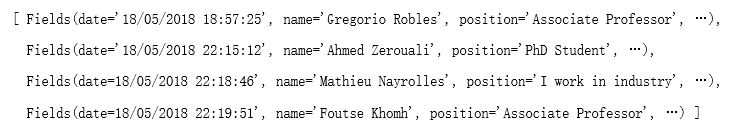
\includegraphics[width=17cm, keepaspectratio]{img/ejemplo45real2}
	\caption{Ejemplo NamedTuple}
	\label{fig:ejemplo4_5Namedtuple}
\end{figure}


En este caso, el NamedTuple se llama \textit{Fields}. Los nombres de los campos hay que definirlos antes de generar el NamedTuple. Una vez tenemos definido el NamedTuple, podemos referirnos a cada campo de éste con su nombre (si tuviesemos un array, tendríamos que saber en qué posición está el campo al que queremos referirnos para llamarlo). Por ejemplo, si del ejemplo anterior de la figura \ref{fig:ejemplo4_5Namedtuple} tenemos guardado el primer NamedTuple en una variable llamada \textit{row}, podremos acceder al nombre de la persona usando (\verb"row.name").


\section{Proceso de tratamiento de información}
\label{sec:tratainfo}
Antes de generar el documento Latex con la información que se ha extraido de la hoja de cálculo, hay que revisar toda esa información que tenemos, y ver si hay que hacer alguna modificación, o no usar literalmente el texto que tenemos en un campo.


\subsection{Ordenar alfabéticamente}
\label{subsec:orden}
Como en este caso tratamos con datos personales, hay que definir un orden de aparición, y para considerar a todos los participantes por igual, sin preferencias, ordenaremos a las personas alfabéticamente.\\

Para esto, se extrae el apellido de cada nombre, y se guardan en un array. Este array es ordenado alfabéticamente con el método de Python \textit{sort}. Con la ayuda de un bucle y del array ordenado, se creará una nueva lista con todos los NamedTuples de datos ordenado alfabéticamente por el apellido del participante.


\subsection{Convertir caracteres especiales}
\label{subsec:especialCars}
Como la intención de este proyecto es generar un documento en Latex, hay que adaptarlo para ello. Latex tiene una serie de caracteres que utiliza para funciones especiales, tales como \textbackslash, \$, \%..., y para que al generar el PDF estos caracteres aparezcan correctamente, tienen que aparecer modificados en el documento Latex.\\

Para solucionar este problema, revisaremos todos los campos en busca de estos caracteres (\$, \#, \%, \&, \^,	\_, \{, \}, \~, \textbackslash) y cuando los encuentre, añadirá delante de ellos un \textit{backslash} (\textbackslash). De esta forma, aparecerá el caracter deseado, y no generará errores y confusiones a la hora de generar el PDF final.\\

Hay algunos casos especiales en los que no conviene hacer este proceso. Por ejemplo, si uno de los campos es una URL, y dicha URL no la vamos a escribir literalmente en el documento final, sino que la vamos a utilizar para obtener otro dato. En este caso tenemos, por ejemplo, un campo que corresponde a la URL de una imagen (se explicará a continuación), y esta URL será utilizada para descargar la imagen correspondiente, por tanto si hacemos el proceso anterior sobre la URL, cuando la utilicemos en el programa será incorrecta, por lo que no hay que modificarla.


\subsection{Descarga de imágenes personales}
\label{subsec:imagenes}


\subsection{Obtener banderas de nacionalidad}
\label{subsec:banderas}


\subsection{Acortar presentaciones}
\label{subsec:presentacion}


\subsection{Imágenes de hiring y looking}
\label{subsec:imaghiringlooking}
??????


\section{Creación de la sección de participantes en Latex}
\label{sec:creaParticipantes}


\section{Guarda el fichero Latex con los datos}
\label{sec:guardaLatex}



\section{Busca fichero intro.tex}
\label{sec:ficheroIntro}


%%%%%%%%%%%%%%%%%%%%%%%%%%%%%%%%%%%%%%%%%%%%%%%%%%%%%%%%%%%%%%%%%%%%%%%%%%%%%%%%
%%%%%%%%%%%%%%%%%%%%%%%%%%%%%%%%%%%%%%%%%%%%%%%%%%%%%%%%%%%%%%%%%%%%%%%%%%%%%%%%
% RESULTADOS %
%%%%%%%%%%%%%%%%%%%%%%%%%%%%%%%%%%%%%%%%%%%%%%%%%%%%%%%%%%%%%%%%%%%%%%%%%%%%%%%%

\cleardoublepage
\chapter{Resultados}

En este capítulo se incluyen los resultados de tu trabajo fin de grado.

Si es una herramienta de análisis lo que has realizado, aquí puedes poner ejemplos de haberla utilizado para que se vea su utilidad.


%%%%%%%%%%%%%%%%%%%%%%%%%%%%%%%%%%%%%%%%%%%%%%%%%%%%%%%%%%%%%%%%%%%%%%%%%%%%%%%%
%%%%%%%%%%%%%%%%%%%%%%%%%%%%%%%%%%%%%%%%%%%%%%%%%%%%%%%%%%%%%%%%%%%%%%%%%%%%%%%%
% CONCLUSIONES %
%%%%%%%%%%%%%%%%%%%%%%%%%%%%%%%%%%%%%%%%%%%%%%%%%%%%%%%%%%%%%%%%%%%%%%%%%%%%%%%%

\cleardoublepage
\chapter{Conclusiones}
\label{chap:conclusiones}


\section{Consecución de objetivos}
\label{sec:consecucion-objetivos}

Esta sección es la sección espejo de las dos primeras del capítulo de objetivos, donde se planteaba el objetivo general y se elaboraban los específicos.

Es aquí donde hay que debatir qué se ha conseguido y qué no.
Cuando algo no se ha conseguido, se ha de justificar, en términos de qué problemas se han encontrado y qué medidas se han tomado para mitigar esos problemas.


\section{Aplicación de lo aprendido}
\label{sec:aplicacion}

Aquí viene lo que has aprendido durante el Grado/Máster y que has aplicado en el TFG/TFM. Una buena idea es poner las asignaturas más relacionadas y comentar en un párrafo los conocimientos y habilidades puestos en práctica.

\begin{enumerate}
  \item a
  \item b
\end{enumerate}


\section{Lecciones aprendidas}
\label{sec:lecciones_aprendidas}

Aquí viene lo que has aprendido en el Trabajo Fin de Grado/Máster.

\begin{enumerate}
  \item a
  \item b
\end{enumerate}


\section{Trabajos futuros}
\label{sec:trabajos_futuros}

Ningún software se termina, así que aquí vienen ideas y funcionalidades que estaría bien tener implementadas en el futuro.

Es un apartado que sirve para dar ideas de cara a futuros TFGs/TFMs.


%%%%%%%%%%%%%%%%%%%%%%%%%%%%%%%%%%%%%%%%%%%%%%%%%%%%%%%%%%%%%%%%%%%%%%%%%%%%%%%%
%%%%%%%%%%%%%%%%%%%%%%%%%%%%%%%%%%%%%%%%%%%%%%%%%%%%%%%%%%%%%%%%%%%%%%%%%%%%%%%%
% APÉNDICE(S) %
%%%%%%%%%%%%%%%%%%%%%%%%%%%%%%%%%%%%%%%%%%%%%%%%%%%%%%%%%%%%%%%%%%%%%%%%%%%%%%%%

\cleardoublepage
\appendix
\chapter{Manual de usuario}
\label{app:manual}


%%%%%%%%%%%%%%%%%%%%%%%%%%%%%%%%%%%%%%%%%%%%%%%%%%%%%%%%%%%%%%%%%%%%%%%%%%%%%%%%
%%%%%%%%%%%%%%%%%%%%%%%%%%%%%%%%%%%%%%%%%%%%%%%%%%%%%%%%%%%%%%%%%%%%%%%%%%%%%%%%
% BIBLIOGRAFIA %
%%%%%%%%%%%%%%%%%%%%%%%%%%%%%%%%%%%%%%%%%%%%%%%%%%%%%%%%%%%%%%%%%%%%%%%%%%%%%%%%

\cleardoublepage

% Las siguientes dos instrucciones es todo lo que necesitas
% para incluir las citas en la memoria
\bibliographystyle{abbrv}
\bibliography{memoria}  % memoria.bib es el nombre del fichero que contiene
% las referencias bibliogríficas. Abre ese fichero y mira el formato que tiene,
% que se conoce como BibTeX. Hay muchos sitios que exportan referencias en
% formato BibTeX. Prueba a buscar en http://scholar.google.com por referencias
% y verás que lo puedes hacer de manera sencilla.
% Más información:
% http://texblog.org/2014/04/22/using-google-scholar-to-download-bibtex-citations/

\end{document}
